\documentclass{scrartcl}
\usepackage[utf8]{inputenc}
\usepackage{bussproofs}
\usepackage{scrpage2}
\usepackage{rotating}
\usepackage{listings}
\usepackage{amsmath}
\usepackage{amsfonts}
%\usepackage{mathtools}
\usepackage{hyperref}
\pagestyle{scrheadings}
\renewcommand{\thesubsection}{\alph{subsection}}
\clearscrheadfoot
\ohead[]{Nikolas Zeitler, Joshua Hartmann, Alexander Diegel}
\cfoot[\pagemark]{\pagemark}
\author{Nikolas Zeitler, Joshua Hartmann, Alexander Diegel}
\title{Maschinelles Lernen Blatt 3}

\begin{document}
\maketitle
\subsection*{a)Einlesen der Daten.} siehe Matlab-File.
\subsection*{b) Die Daten zu jeder Kenngröße jeder Schwertlilienart aus den Trainingsdaten sollen in einem Histogramm veranschaulicht werden. Höchstens sechs Sätze sollen zudem Auffälligkeiten in den Daten beschreiben}

\begin{tabular}{ccc}
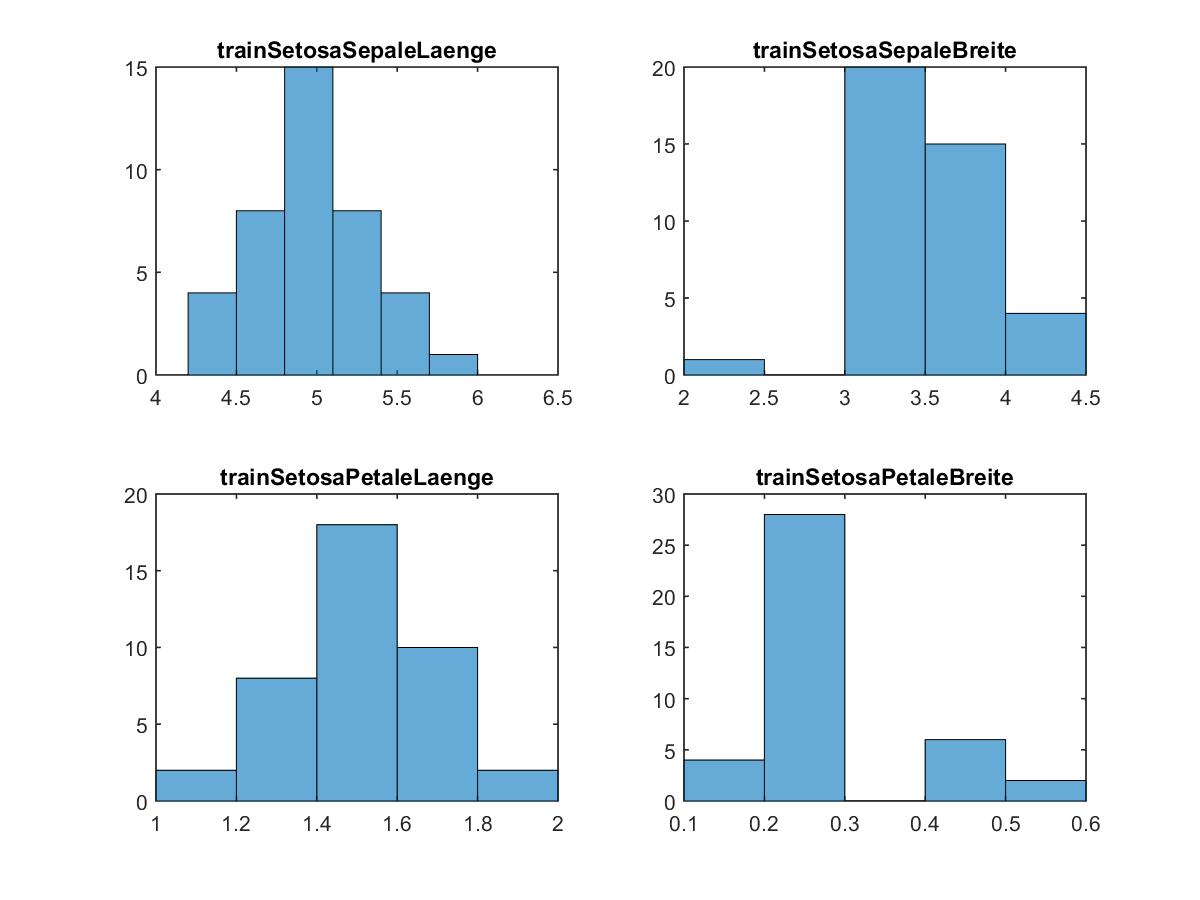
\includegraphics[width=0.3\textwidth]{plots/trainSetosa.jpg}  &
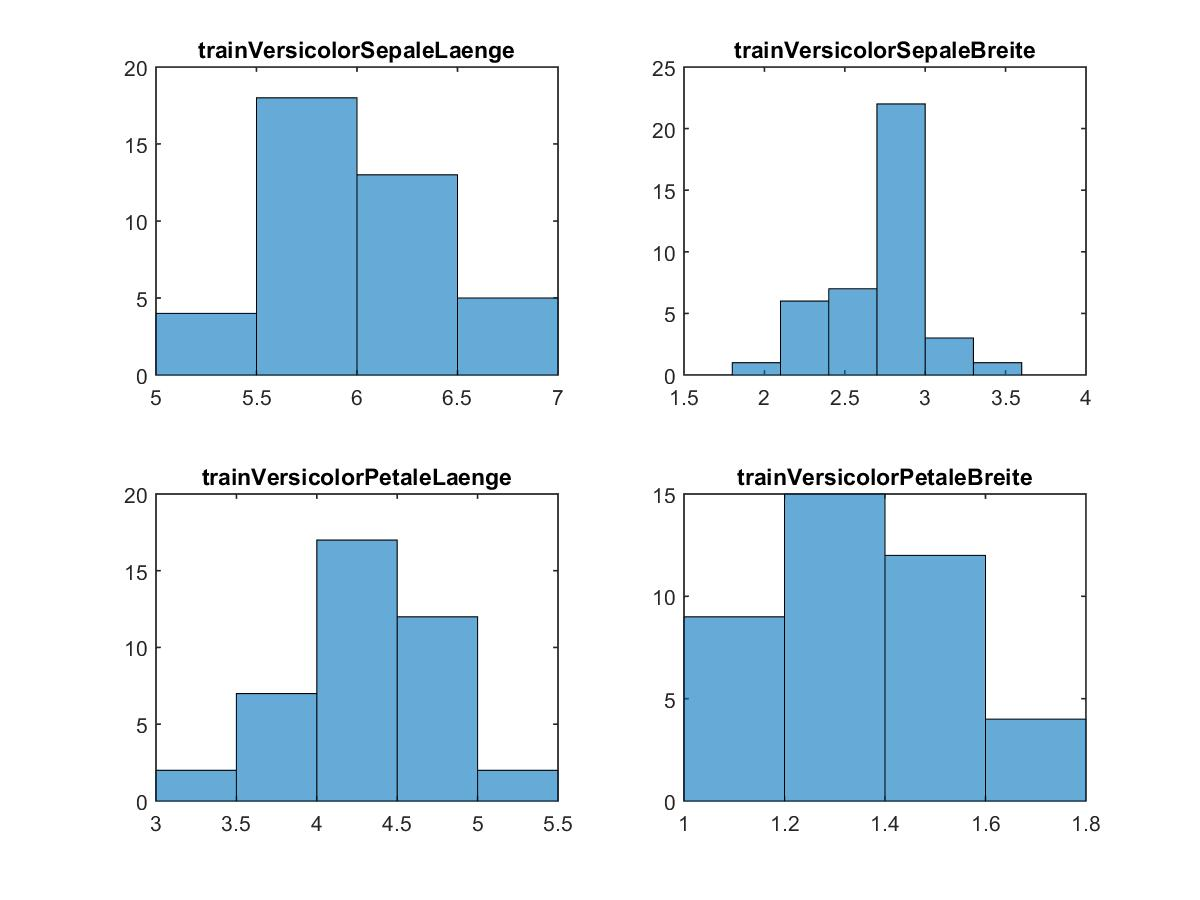
\includegraphics[width=0.3\textwidth]{plots/trainVersicolor.jpg} & 
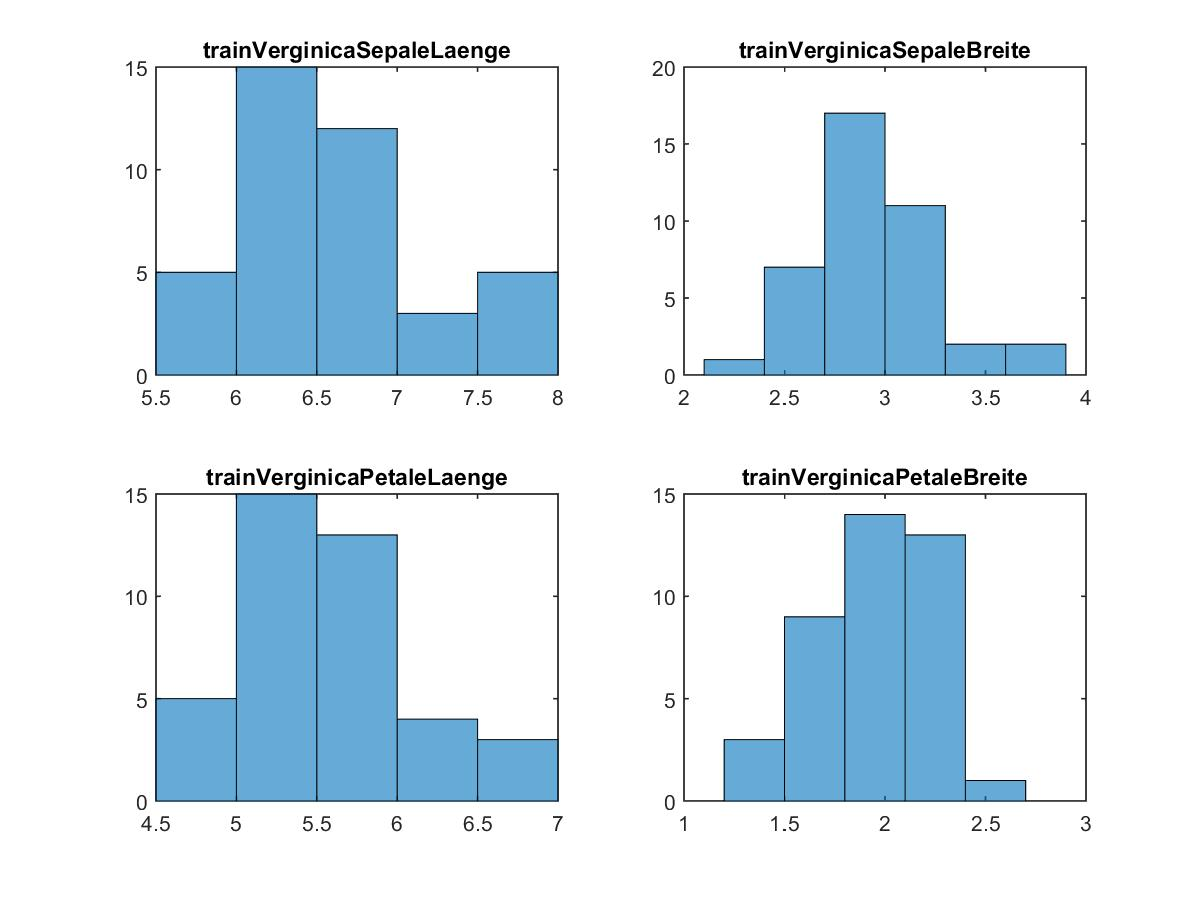
\includegraphics[width=0.3\textwidth]{plots/trainVerginica.jpg} 

\end{tabular}
	
Die meisten Histogramme ähneln einer gauss'schen Normalverteilung.
Die Gattung Setosa bildet hinsichtlich der sepalen Länge die kleinste Art (der Erwartungswert dieser Größe ist ca. 5, wie in Aufgabe c) dargestellt wird, Verginica hat für diese Größe mit 6.6 den größten Erwartungswert). \\
Bei der Gattung Setosa gibt es eine Lücke in den Histogrammen für die sepale und petale Breite- während es bei der sepalen Länge Zufall sein kann, dass zwischen 2,5 und 3 keine Werte gemessen wurden (vllt. hätte man einfach mehr Messungen durchführen müssen), ist die Lücke bei der petalen Breite auffälliger, da hier ein Wert zwischen 27 und 7 erwartet werden würde (ginge man von einer Normalverteilung dieser Eigenschaft aus).\\
Ebenfalls die mit Abstand kleinste Art ist die Setosa für die petale Breite.\\
Die Gattung Versicolor hat einen großen Ausschlag bei der sepalen Breite (ca. bei 2,75-3 sie ist die kleinste der drei Arten für dieses Merkmal). \\
Die Gattung Verginica ist die größte aller drei Arten bei allen Merkmalen (wenn die Erwartungswerte betrachtet werden.) Sie hat aber u.a. das breiteste Spektrum z.B. bei der sepalen Länge. 

%TODO TEAM: Muss hier noch mehr hin? Bzw. was fällt euch noch an den Daten auf, das man hier schreiben könnte?
\subsection*{c)Für jede Kenngröße jeder Schwertlilienart sind anschließend sowohl der Mittelwert als auch die Varianz	für die Trainingsdaten zu bestimmen.}

Kenngrößen in der Reihenfolge, wie sie auch in den gegebenen Dateien vorliegen.\\

meanSetosa $ = [5.04, 3.54, 1.47, 0.25]$ \\
meanVersicolor  $ = [5.9, 2.75,	4.2, 1.3]$ \\
meanVerginica $ = [6.592, 2.98, 	5.4975, 2.022]$ \\ 

varSetosa $ = [0.13,	0.15,	0.035,	0.012]$ \\
varVersicolor $ = [0.2, 0.09, 0.22, 0.04]$\\
varVerginica $ = [0.36, 0.1, 0.3, 0.08]$ \\
\subsection*{d)Likelihoods sowie Bayes'sche Klassifikation - siehe Matlab-File}
%\begin{tabular}{ccc}
%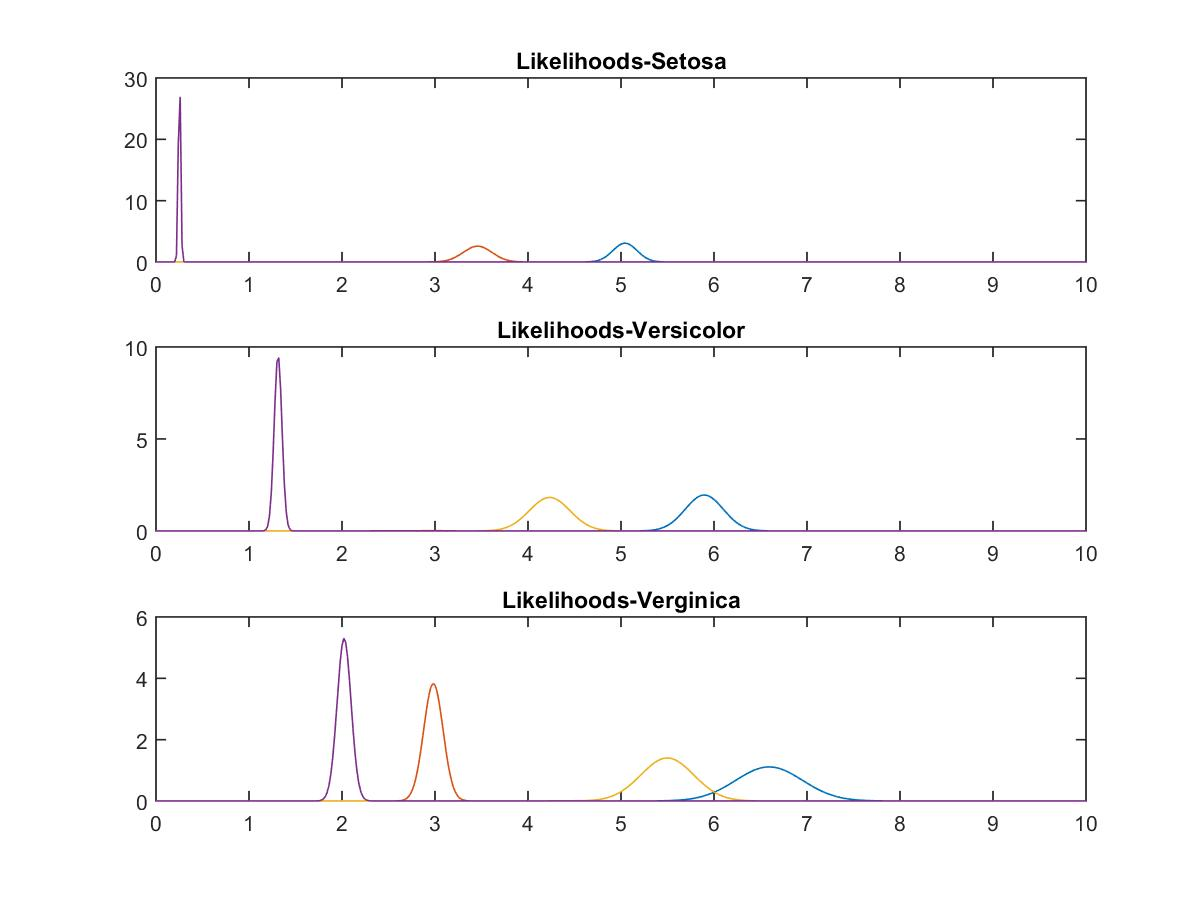
\includegraphics[width=0.45\textwidth]{plots/LikelihoodsAll.jpg} &
%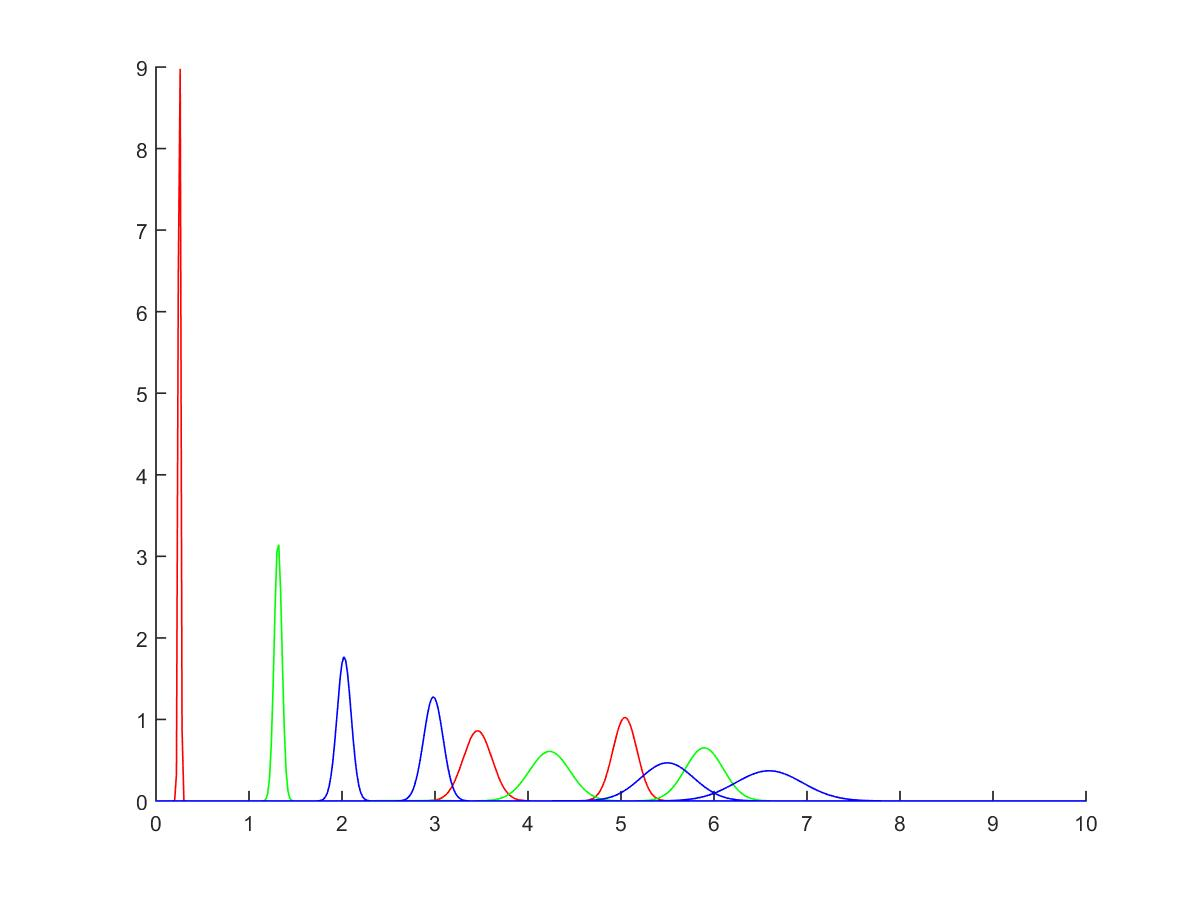
\includegraphics[width=0.45\textwidth]{plots/BayesAll.jpg}
%\end{tabular}
\section*{e) Maßzahlen}
\begin{tabular}{|c|c|c|c|}
	\hline
	&	Setosa	&	Versicolor	&	Verginica\\ 
	\hline
	true positive  & 10	&9	&9\\
	true negative  & 20	&19	&19\\
	false positive & 0	&1	&1\\
	false negative & 0	&1	&1\\
	\hline
\end{tabular}

\subsection*{f)Kenngrößen}
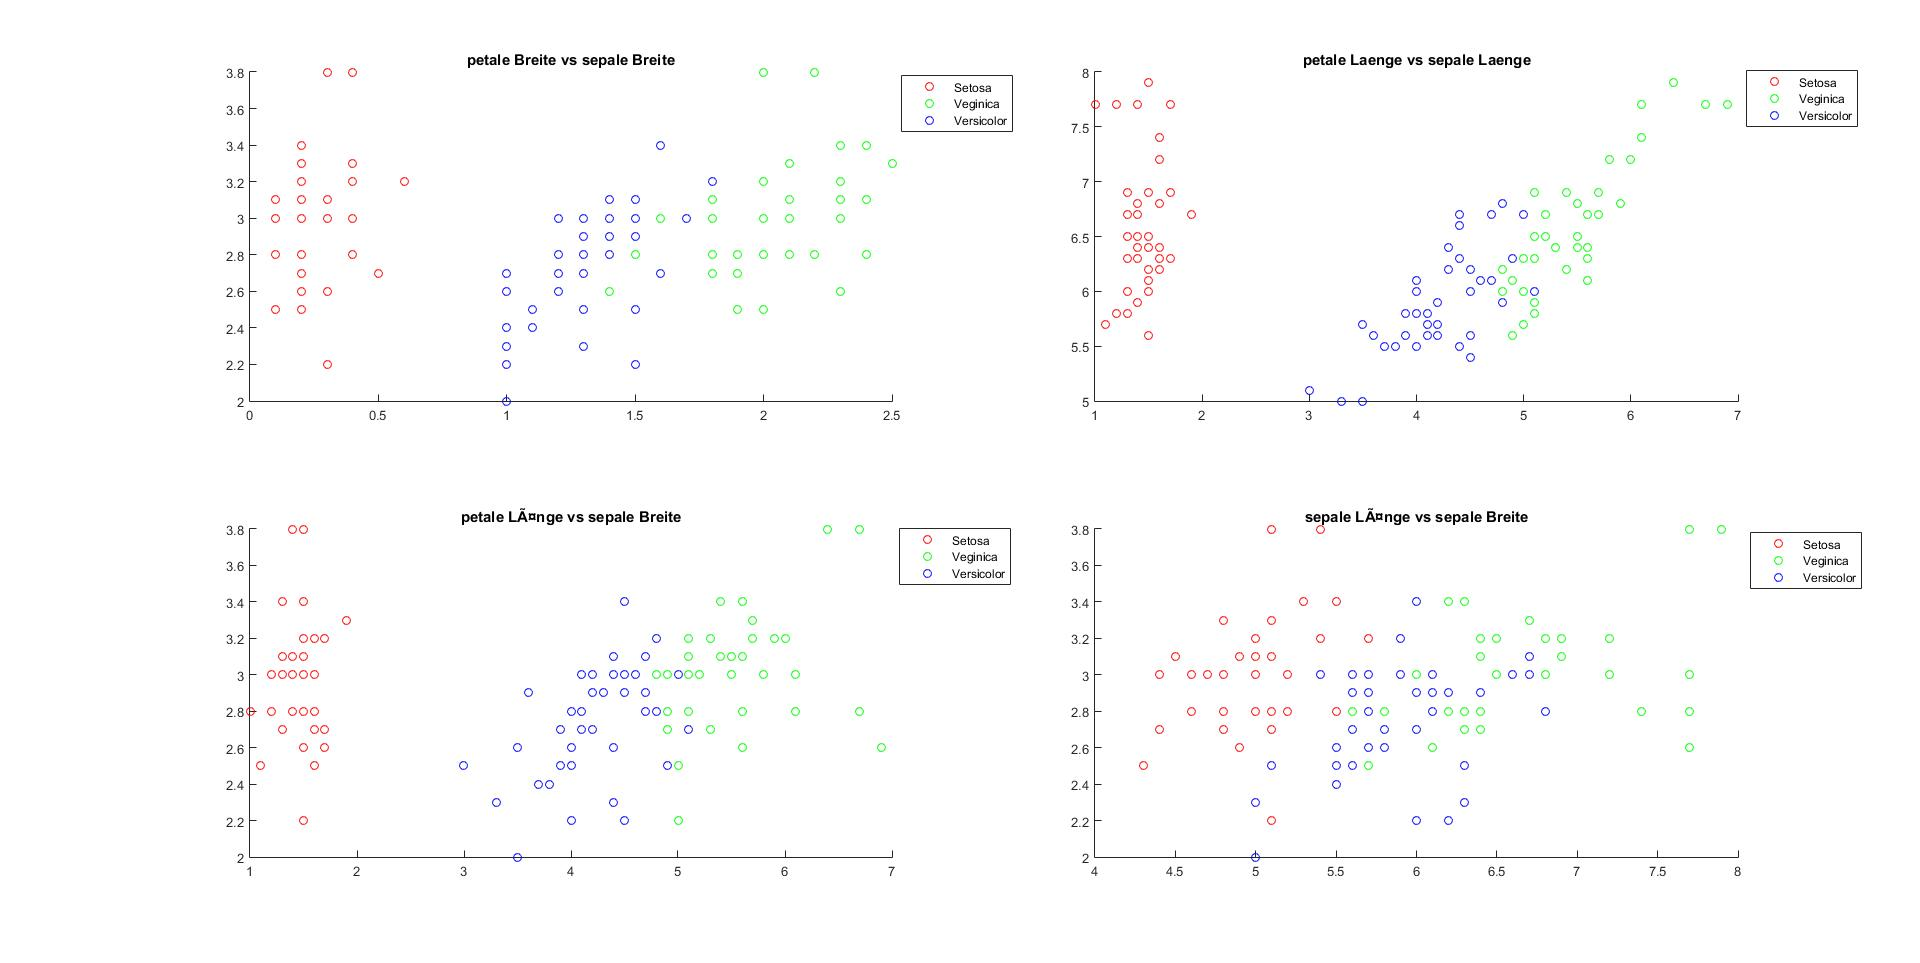
\includegraphics[width=1.1\textwidth]{plots/plotF.jpg} \\ 

Die Gattung Setosa ist gut gegenüber den anderen Arten in den ersten drei Plots abzugrenzen.
Das kommt daher, dass diese Pflanze die schmalste ist. \\
Beim Plot sepale Länge vs. sepale Breite ist die Unterscheidung nicht mehr ganz so deutlich zu erkennen, das kommt daher, dass sich die sepalen Längen und Breite aller drei Arten zum Teil überschneiden.\\
Dieser Plot zeigt des Weiteren Unterscheidungsschwierigkeiten zwischen Verginica und Versicolor auf. \\
Diese Durchmischung zeigt sich bereits teilweise in den ersten drei Plots, wird in diesem aber besonders deutlich. \\
Das liegt daran, dass sich Verginica und Versicolor (bzw. deren Wertebereiche in den folgenden Eigenschaften) bei sepaler Länge und Breite sowie petaler Länge ähnlich sind (es gibt Überschneidungen).\\
Die isolierte Betrachtung von den Kenngrößen würde also keine besonders zuverlässige Klassifizierung liefern.

dsfsdf
% müsste jetzt alles mehr oder weniger im text stehen, wenn nicht: nachtragen! (den letzten Satz verstehe ich nicht)
%3: Auffallend ist das man immer einige wenige überschneidungen zwischen Veginica und Versicolor hat, eine eindeutige unterscheidung ausschließlich an hand der sepalen maße wird wohl schwer fallen. \\
%4: Man kann hoffen das diese wenigen überschneidungen immer andere Pflanzen sind, dann könnte es möglich sein mit hilfe der übrigen Plots ein eindeutiges Ergebnis zu erhalten

\subsection*{g) Multivariate Normalverteilung- siehe Matlab-File}

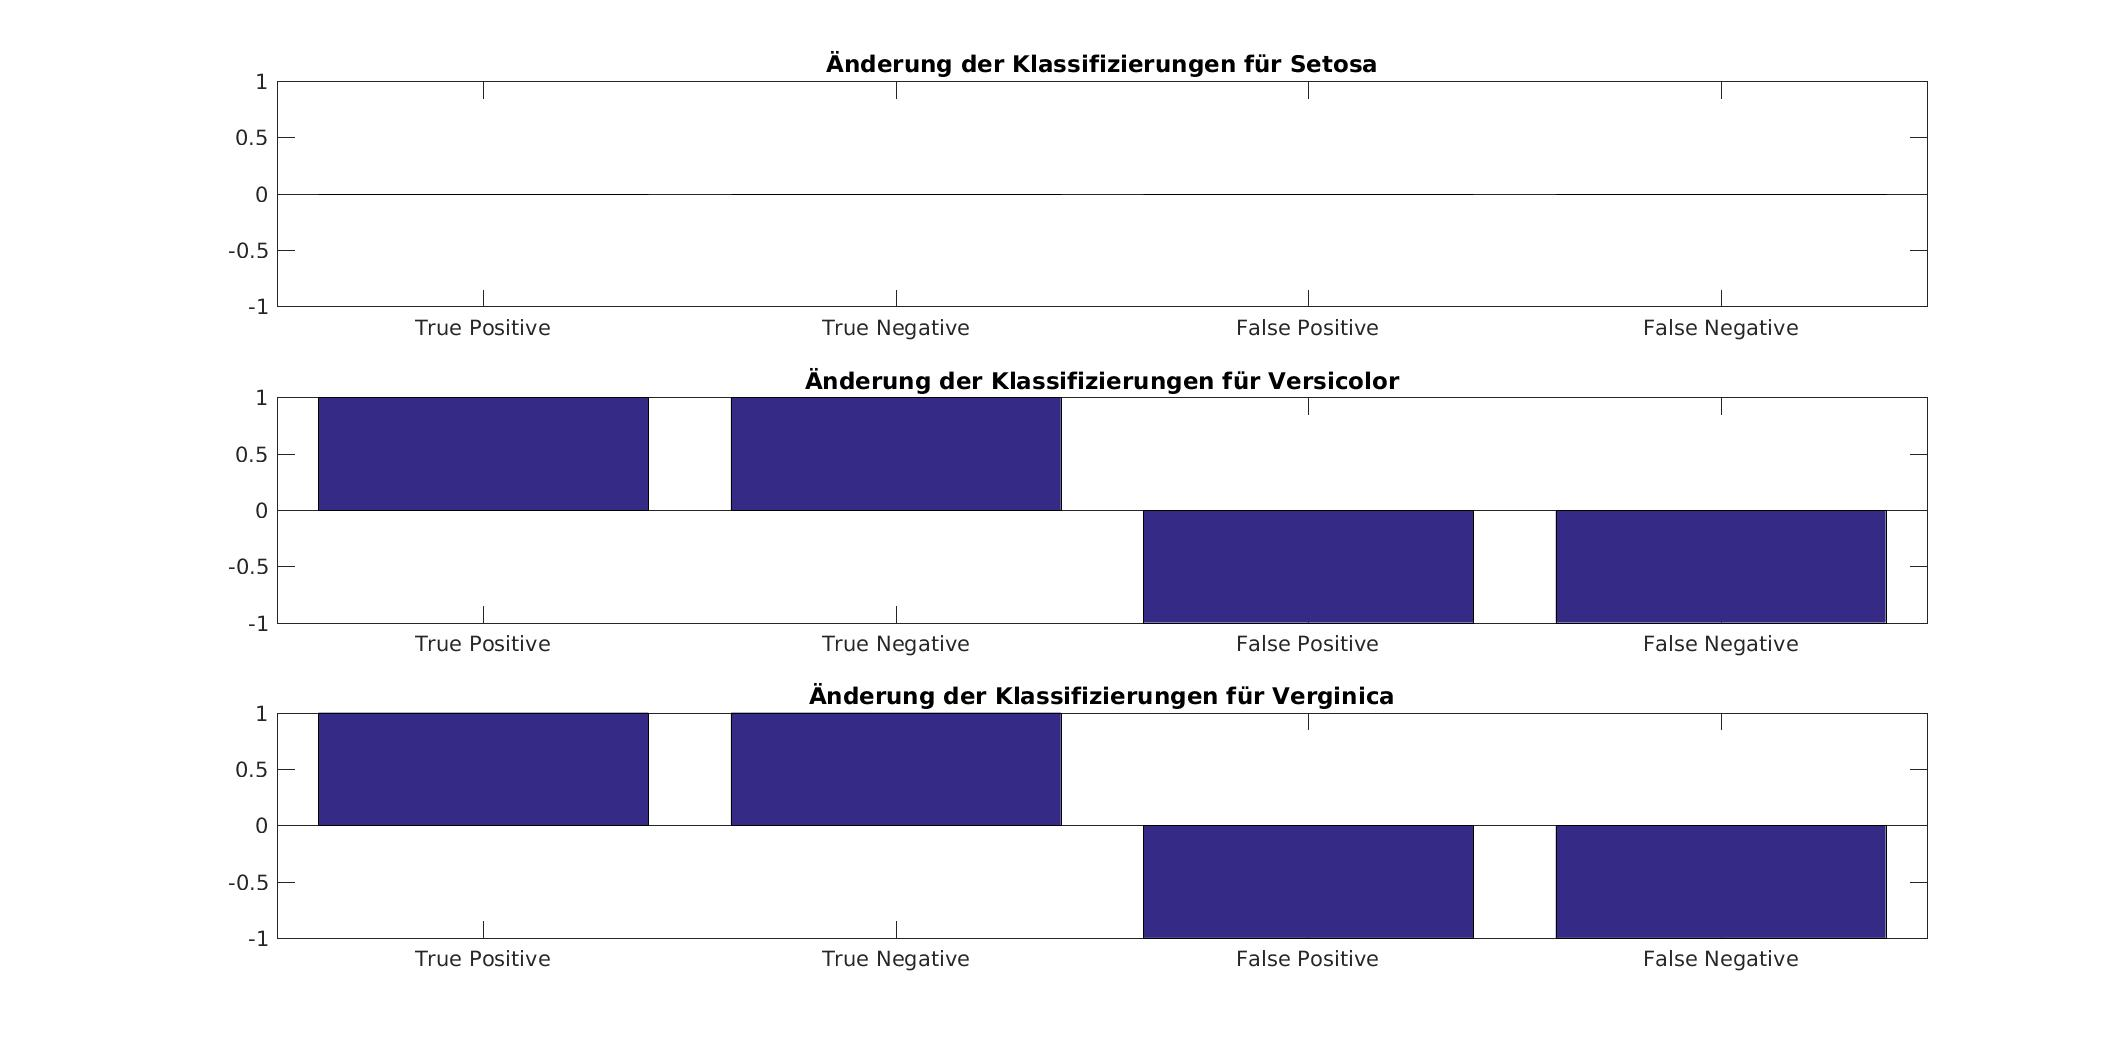
\includegraphics[width=0.9\textwidth]{plots/diffsAll.jpg} \\

Wir haben uns dafür entschieden, die Änderungen der Anzahl der Datenpunkte für True Positive, True Negative, False Positive und False Neagative aufzutragen.\\
Damit zeigt sich direkt die Änderung der Klassifizierung der Testdaten.

\subsubsection*{Erklärung der Änderungen:}

Nach der Klassifikation mit der Annahme, dass es sich bei den Kenngrößen um eine multivariate Normalverteilung (und keine unabhängigen Daten) handelt, konnten alle Schwertlinien korrekt klassifiziert werden.
Die getroffene Annahme, dass die einzelnen Kenngrößen stochastisch abhängig sind, scheint die Realität besser zu entsprechen.

Zuvor wurden geringe Klassifikationsfehler  bei Versicolor und Verginica gemacht (10\% bzw. 5\%). (Diese Aussagen sind jedoch mit Vorsicht zu genießen, da es sich um einen sehr kleinen Testdatensatz handelt.)
\end{document}
